\section{Introduction}

\begin{frame}
  \frametitle{Are Typesystems Useful?}
  
  \begin{itemize}
    \item advent of DSLs and DSL tools made writing languages popular
    \item easy even for complex domains
    \item complex languages require complex constraint checking
    \item most languages have a concept of \textbf{type}: reusable building
    blocks for constraints
  \end{itemize}
  
  In this presentation:
  \begin{itemize}
    \item Using Xtext as DSL development environment
    \item case study: form based editing of entities
    \item compare different approaches to use type systems
  \end{itemize}
\end{frame}

\begin{frame}
	\frametitle{Case Study} % for adjustments use overpic[grid,tics=10]  
	\begin{overpic}[scale=0.6]%
       {img/form-valid.png}
       \only<2>{
        \put(55,-40){\includegraphics[scale=0.6]%
		{img/form-invalid.png}}}
     \end{overpic}
	
	
%	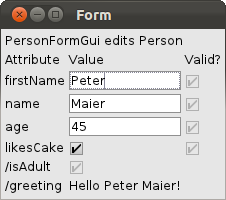
\includegraphics[width=0.5\linewidth]{img/form-valid.png}
	%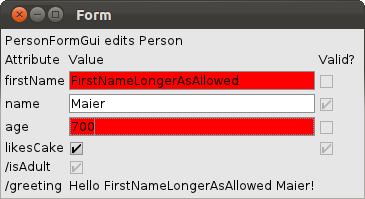
\includegraphics[width=0.7\linewidth]{img/form-invalid.png}
\end{frame}

\begin{frame}[allowframebreaks,fragile]
  \frametitle{Typesystem Introduction}
  \begin{itemize}
    \item Concept of types
    \item static vs dynamic type checking
  \end{itemize}

  \begin{itemize}
    \item graphical example for type inference
   \end{itemize}

\begin{small}
\begin{verbatim}
name : string;
num = 41 + 1;
greeting : string = "Hi " + name + 
    ", the answer is " + num + ".";
\end{verbatim}
\end{small}

Common tasks of type systems:

\begin{itemize}
  \item Assigning fixed types to language elements
  \item Subtyping: is a type conformant to another type?
  \item Inferring types of complex expressions
\end{itemize}

\end{frame}

